\chapter{Structure}\label{ch:ekg-mm-structure}

The \glsfirst{ekgmm} is a collection of capabilities structured in a relatively simple 4x5 matrix of
"capability domains" and "maturity levels".

\begin{figure}[ht]
    \centering
    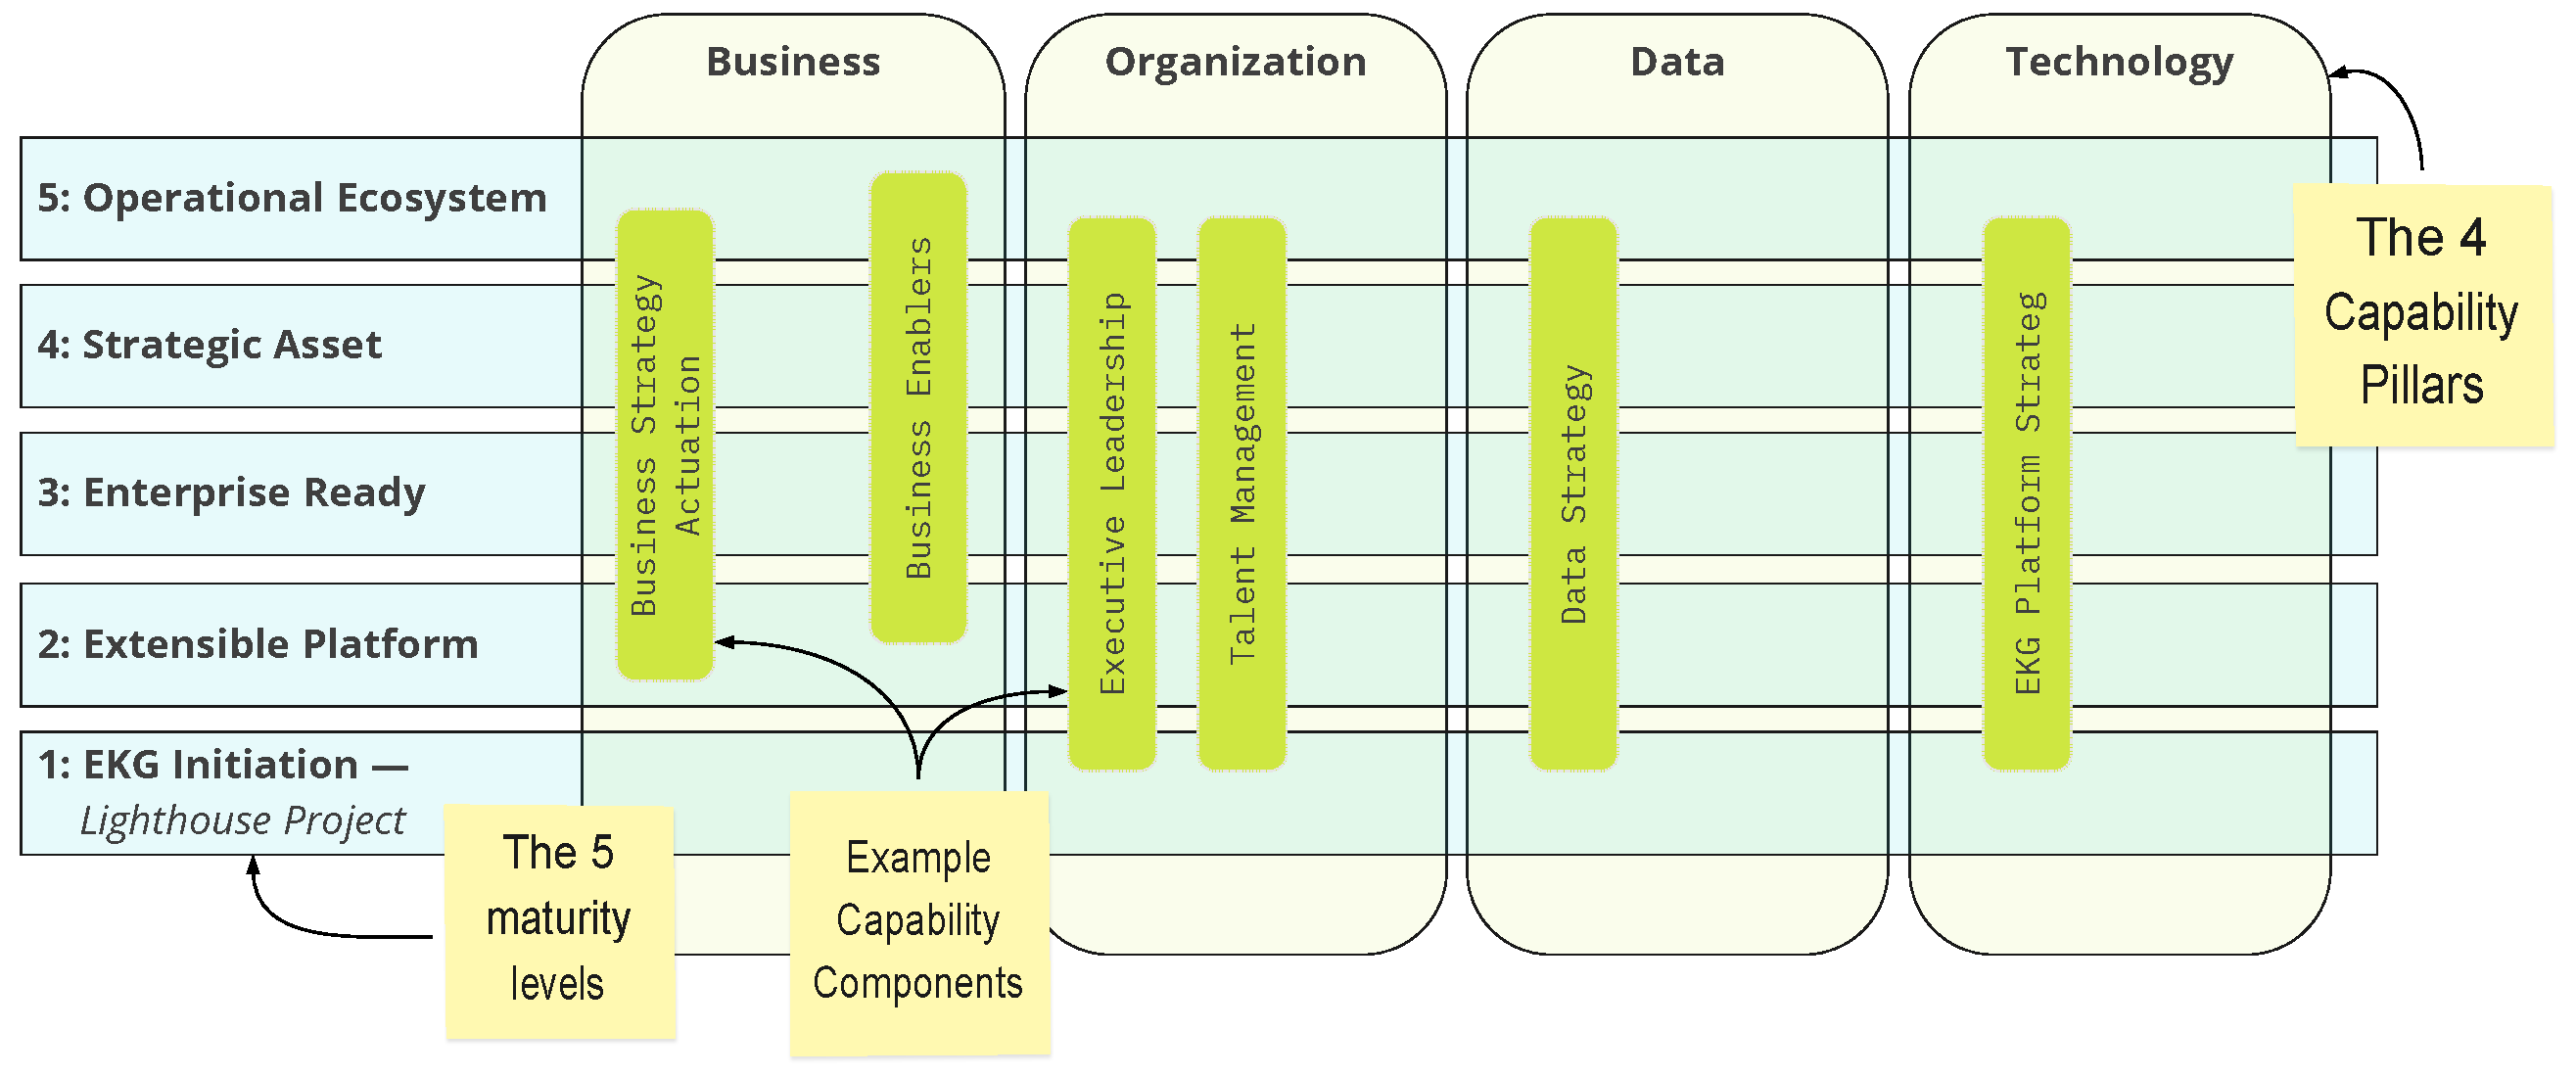
\includegraphics[width=\textwidth]{../images/ekg-mm-structure.pdf}
    \caption{EKG/MM Structure}
    \label{fig:ekg-mm-structure}
\end{figure}

\section{The Four Capability Pillars}\label{sec:ekg-mm-the-four-pillars}
%
% This file is included from various other docs in other repo's, not just EKG/MM itself
%
\label{sec:the-four-capability-domains}
\index{capability domain}
All capabilities that we measure and assess in the \gls{ekgmm}\footnote{See \autocite{ekgmm}} are categorized
in four major categories\,---\,also called "pillars"\,---\,that match the four primary audiences that are involved:

The Business (Strategy) is leading.
In a "Data-centric"\index{data!centric} organization, Data Strategy\index{data!strategy} comes second and
fully supports the Business Strategy\index{business!strategy}.
Then derived from that we have a supporting and facilitating Technology and Organizational Strategy.
\index{strategy!business strategy}
\index{strategy!data strategy}
\index{strategy!technology strategy}
\index{strategy!organization strategy}

These four pillars roughly correspond with the four primary audiences that we are addressing:

\begin{enumerate}
    \item The audience of people on the business-side
    \item The audience of people in the data-management and data-governance departments
    \item The audience of technologists
    \item The audience of people that are project managers, trainers or HR, legal, compliance and finance departments
\end{enumerate}


\subsection{Business Pillar}\label{subsec:ekg-mm-the-four-pillars-business-pillar}

All Business-side capabilities including~\nameref{ch:ekg-mm-business-strategy-actuation},
\index{business!strategy}~\nameref{ch:ekg-mm-business-model-elaboration},
\index{business!architecture!elaboration}~\nameref{ch:ekg-mm-business-enablers}, Alignment,
\nameref{sec:ekg-mm-business-operating-model} and others.
Does not include all the actual Business Capabilities\index{business!capabilities} that
an enterprise may have themselves.

Addresses the \iindex{audience} of personas on the business-side of an enterprise, C-level,
\gls{lob} execs,\index{executive}\index{persona!executive}
corporate planners,\index{corporate planner}\index{persona!corporate planner}
business architects\index{business!architects}, product owners\index{product owner}\index{persona!product owner},
management consultants\index{management consultant}\index{persona!management consultant} and so forth.

\subsection{Organization Pillar}\label{subsec:ekg-mm-the-four-pillars-organization-pillar}

All relevant Organizational Capabilities including~\nameref{ch:ekg-mm-executive-leadership},
~\nameref{ch:ekg-mm-product-ownership},
~\nameref{ch:ekg-mm-delivery-management},
~\nameref{ch:ekg-mm-organizational-culture}, and
~\nameref{ch:ekg-mm-organizational-capabilities}.

Addresses the \iindex{audience} of people that are neither business, data nor tech such as financial execs and experts, risk
execs and experts, program/portfolio/project managers, HR execs and experts and so forth.

\subsection{Data Pillar}\label{subsec:ekg-mm-the-four-pillars-data-pillar}

All Data (Management) capabilities including~\nameref{ch:ekg-mm-data-strategy}.
\index{strategy!data strategy}

Addresses the \iindex{audience} of people in the data-management and data-governance departments.

\subsection{Technology Pillar}\label{subsec:ekg-mm-the-four-pillars-technology-pillar}

All Technology Capabilities including~\nameref{ch:ekg-mm-technology-strategy},
~\nameref{ch:ekg-mm-technology-execution}, and
~\nameref{ch:ekg-mm-user-interface}.
\index{strategy!technology strategy}

Addresses the \iindex{audience} of technologists, technical architects, developers, infrastructure execs and experts,
security execs and experts etc.



\section{The five maturity levels}\label{sec:the-five-maturity-levels}

This document will refer\,---\,for each capability\,---\,to the five maturity levels.

\subsection{Level 1: \ekgmmLevelOneLabel}

The domain of internal \glspl{poc}, pilots or\,---\,ideally\,---\,"\glspl{lighthouse-project}".
The focus is usually on specific targeted baseline use cases constructed using isolated ontologies.
The champions are visionaries who have assembled a specialist team for implementation\,---\,possibly the
start of the \glsfirst{ekg:coe}.
Funding is likely to be project-based and designed to demonstrate capabilities.

\begin{itemize}[leftmargin=1in,font=\bfseries]

    \item[Business]     Stakeholders recognize business opportunities in scaling and amplifying capabilities
                        through \glspl{ekg}.
                        The first internal champion is seeking to socialize strategic business cases,
                        supports innovation, and is willing to take on the disruption challenge.
    \item[Data]         Core data management capabilities (\gls{operating-model}, inventory, data architecture,
                        \hyperref[sec:ekg-mm-vocabularies]{vocabularies, business glossary or terminology},
                        pipeline management, etc.) are being performed.
                        Specific use cases are being implemented with specialist teams for the pilot initiative.
    \item[Technology]   Technology strategy is focused on experimentation and innovation.
                        Manual data transformation and targeted ETL is underway for the pilot.
                        Limited infrastructure and dedicated efforts to build initial knowledge graph components.
    \item[Organization] Champions are internal visionaries who have assembled a specialist team for implementation.
                        The pilot is sanctioned and funded.
                        Knowledge acceleration is being addressed.
                        Overall organizational support is emerging
\end{itemize}

\subsection{Level 2: \ekgmmLevelTwoLabel}

The domain of parallel knowledge graph activities, implementing multiple (related) use cases on the same platform.
The organization is creating reusable architecture\,---\,i.e. "the \gls{ekg:platform}"\,---\,based
on \citefield{ekgprinciples}{title}.
The \glsfirst{ekg:coe} is created.
Funding is likely to be at the \gls{lob} level and starts to (partly) come from \gls{bau} budgets.

\begin{itemize}[leftmargin=1in,font=\bfseries]

    \item[Business]     Stakeholders adopt a “knowledge-centric” mindset in their tactics to strengthen focus on
                        strategic business value.
                        Management elevates the knowledge graph as an organizational and funding priority.
    \item[Data]         Critical data elements are prioritized in the ontology.
                        Approach to identity and meaning resolution is established.
                        Use case trees are defined and modeled to capture shared data relationships.
                        The knowledge graph is becoming the central point for integration.
    \item[Technology]   Reusable architecture based on \citefield{ekgprinciples}{title}.
                        Core software development design approaches are being established and incorporated
                        into strategy.
                        CTO focuses on extending pilot initiatives for additional leverage.
    \item[Organization] \Gls{operating-model} of collaboration is implemented to support the knowledge graph.
                        The Center of Excellence and DataOps environment is initiated.
                        Budget and implementation strategy are based on agile and synchronized with the
                        use case tree methodology.
\end{itemize}

\subsection{Level 3: \ekgmmLevelThreeLabel}

The establishment of a secure, scalable and resilient \gls{ekg:platform} for business-critical strategic use cases.
Resources for the design and build of operational systems are defined and coordinated.
The knowledge graph is now really an \myuline{Enterprise} Knowledge Graph (EKG) that serves as the
semantic data fabric\index{data fabric} for the organization.
Ownership, governance, and funding are managed at the enterprise level and coordinated by the \gls{ekg:coe} that
oversees the full life-cycle of use cases from inception to deployment and beyond.
Long-term "operate \& optimize" processes are in place.

\begin{itemize}[leftmargin=1in,font=\bfseries]

    \item[Business]     Strong collaboration between various business and support units to prioritize
                        strategic business cases.
    \item[Data]         Inventory is embedded into the \gls{ekg} and linked to governance.
                        Data is expressed as formal ontologies, onboarded into the \gls{ekg} and searchable.
                        Data flows are defined and modeled.
                        The \gls{ekg} is the authoritative source for data.
    \item[Technology]   Commitment to the \gls{ekg} as the strategic infrastructure for the organization.
                        IaC and continuous deployment adopted and implemented.
                        Cloud architecture defined for elasticity.
                        Datapoint security and authentication processes implemented
    \item[Organization] The \gls{ekg} is recognized as a core service for the enterprise.
                        Enterprise-wide ownership and funding processes are operational.
                        The \gls{ekg:coe} is a stand-alone \gls{bau} department.
\end{itemize}

\subsection{Level 4: \ekgmmLevelFourLabel}

The \gls{ekg} is understood as strategic infrastructure\,---\,as an operational utility\,---\,for the organization
and the authoritative source for most data (except for data that originates from core legacy systems).
It supports structural application rationalization\index{rationalization}, high-level and high-quality \gls{ai}
that can take over many tasks from humans and process automation.
Strategic funding is based on the vision of executive management and fully embraced by the Board of Directors.
All core data management capabilities have been achieved.

\subsection{Level 5: \ekgmmLevelFiveLabel}

The \gls{ekg} is central to systems and business processes.
It has been fully integrated into both internal operations and external supply chain partners.
Workflows and approval steps are fully automated.
Entitlements and access rights are controlled by the \gls{ekg}.
Inference and reasoning capabilities are used for advanced \gls{ai} use cases.


\todo[inline]{TODO: How to use the model?}

\todo[inline]{TODO: Can be used for?}

\todo[inline]{TODO: Benchmarking industry}


